\section{tasks::subtract\-Sky\-N Class Reference}
\label{classtasks_1_1subtractSkyN}\index{tasks::subtractSkyN@{tasks::subtractSkyN}}
Inheritance diagram for tasks::subtract\-Sky\-N::\begin{figure}[H]
\begin{center}
\leavevmode
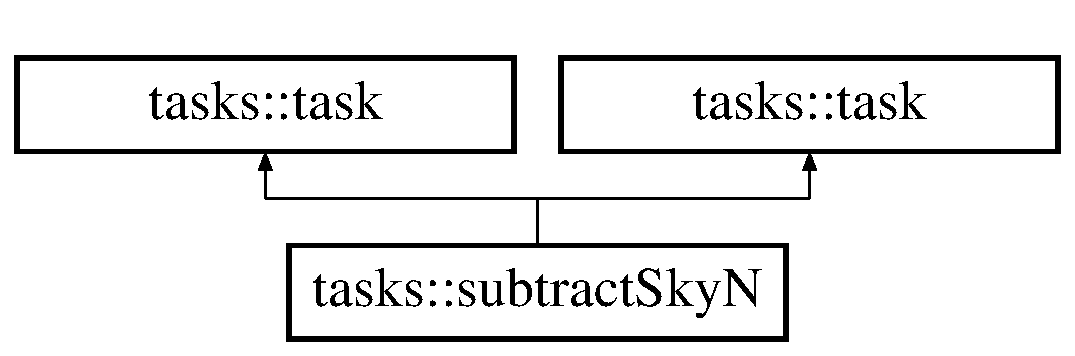
\includegraphics[height=2cm]{classtasks_1_1subtractSkyN}
\end{center}
\end{figure}
\subsection*{Public Member Functions}
\begin{CompactItemize}
\item 
def \textbf{run}\label{classtasks_1_1subtractSkyN_eb683a767a22ed0724c29ef695b1269e}

\item 
def \textbf{run}\label{classtasks_1_1subtractSkyN_eb683a767a22ed0724c29ef695b1269e}

\end{CompactItemize}
\subsection*{Static Public Attributes}
\begin{CompactItemize}
\item 
string \textbf{name} = '{\bfsubtract\-Sky\-N}'\label{classtasks_1_1subtractSkyN_8584fba620680fed12440a401274c339}

\item 
string \textbf{button\-Text} = 'Subtrac sky (N)'\label{classtasks_1_1subtractSkyN_0210339b077a88fbee9fcaa4683fce73}

\end{CompactItemize}


\subsection{Detailed Description}


\footnotesize\begin{verbatim}Subtract sky from an image using N images for sky computing
\end{verbatim}
\normalsize
 



The documentation for this class was generated from the following files:\begin{CompactItemize}
\item 
old/PANICtool-1.0/tasks.py\item 
old/tasks.py\end{CompactItemize}
